\chapter{Cycles as a Vertex Invariant}

A powerful feature of the cycles invariant is that it is not only discriminatory between graphs, it suggests potential isomorphisms between their vertices.
This section will discuss exactly how isomorphisms can be constructed and evaluated by using cycles as a vertex invariant.
Central to this chapter is the concept described earlier as Automorphism Equivalence Classes, or Similar Vertex Sets (SVS).

\section{Perfect Similar Vertex Sets}

A vertex-similar sets is a subset of the vertices of a graph such that for any pair of vertices in the set, there exists an automorphism which maps one to the other.
Note that vertex similarity is reflexive (as one-to-one mapping (such as an automorphism) is invertible). 
Also note that membership in vertex-similar sets is transitive (as we can simply use the `followed-by' operator on the component automorphism mappings).

Thus, all vertices in a graph can be partitioned into some number of similarity-sets, where every set has at least one element, and the union of the sets is the vertex set.
For the sake of simplicity, we will assume that there is some well-ordering over these sets, so that we are able to assign an order to each set within the collection of similar vertex sets.
In practice, this will be a practical function of how we go about computing the SVSes.

This construction is deeply tied to isomorphism checking and discovery.
If we have two graphs $G$ and $H$, and their Similar Vertex Sets are $SVS(G)$ and $SVS(H)$, based on the size of each set, we have a maximum number of potential isomorphisms.
First off, if we examine every $i$th paired set between $SVS(G)[i]$ and  $SVS(H)[i]$, if the sizes of the sets differ, then we can immediately reject the possibility of isomorphism between $G$ and $H$.
If the size of each component set are the same, we can check for isomorphism by brute force, by calculating every possible permutation between the paired sets, and then every combination of those permutations across all of the SVSes.
Though we can make many practical arguments which greatly simplify the number of these possibilities we have to test for isomorphism, it should be noted that in the overwhelming majority of cases, this simple algorithm only has to check \emph{one} mapping for an isomorphism.
This is by virtue of the fact the the overwhelming majority of graphs have only a single automorphism.

\section{Most Graphs Have One Automorphism}

This is by virtue of a simple fact: we can talk broadly about the average number of automorphisms in a set of graphs, and even better, we can calculate precise means for the average number of automorphisms for graphs of a certain size.
Remember that the number of undirected, non-looped, single-edge graphs (or as we have just been calling them, graphs), over N vertices has a known closed form.
We also know that the number of graph instances over N nodes is simply the number of undirected matrices over N nodes, $2^{E_{max}}$.
Finally, we know that the number of matrices 

$$ M_{reps}(g) = \frac{N!}{|Aut(g)|} $$
$$ \sum_{g \in G_{alg}} M_{reps}(g) = \sum_{g \in G_{alg}} \frac{N!}{|Aut(g)|} $$
$$ 2^{\frac{N^2 - N}{2}} = N! \sum_{g \in G_{alg}} \frac{1}{|Aut(g)|} $$
$$\frac{\sum_{g \in G_{alg}} \frac{1}{|Aut(g)|}}{|G_{alg}|} =  \frac{2^{\frac{N^2 - N}{2}}}{N! * |G_{alg}|} $$
$$ \xoverline{|Aut^{-1}(g)|} = \frac{2^{\frac{N^2 - N}{2}}}{N! * |G_{alg}|}$$

Though we don't have a closed form for this, a quick calculation pretty easy, and gives us a very clear trend.
In Figure \ref{fig:mostgraphsoneaut}, there are two figures shown.
The first plot shows the right hand side of the final equation, graphed for different values of N.
The second plot explores the difference between the first plot and one, and takes the logarithm to see how small the values get.

\begin{figure}[h]
\label{fig:mostgraphsoneaut}
\caption{\emph{Most Graphs Have Exactly One Automorphism} - It is clear that as N increases, the right hand side of our above equation approaches 1. Not only that, but it appears to do so exponentially fast.  The plot on the right shows a logarithmic linear approach to one.}
\centering
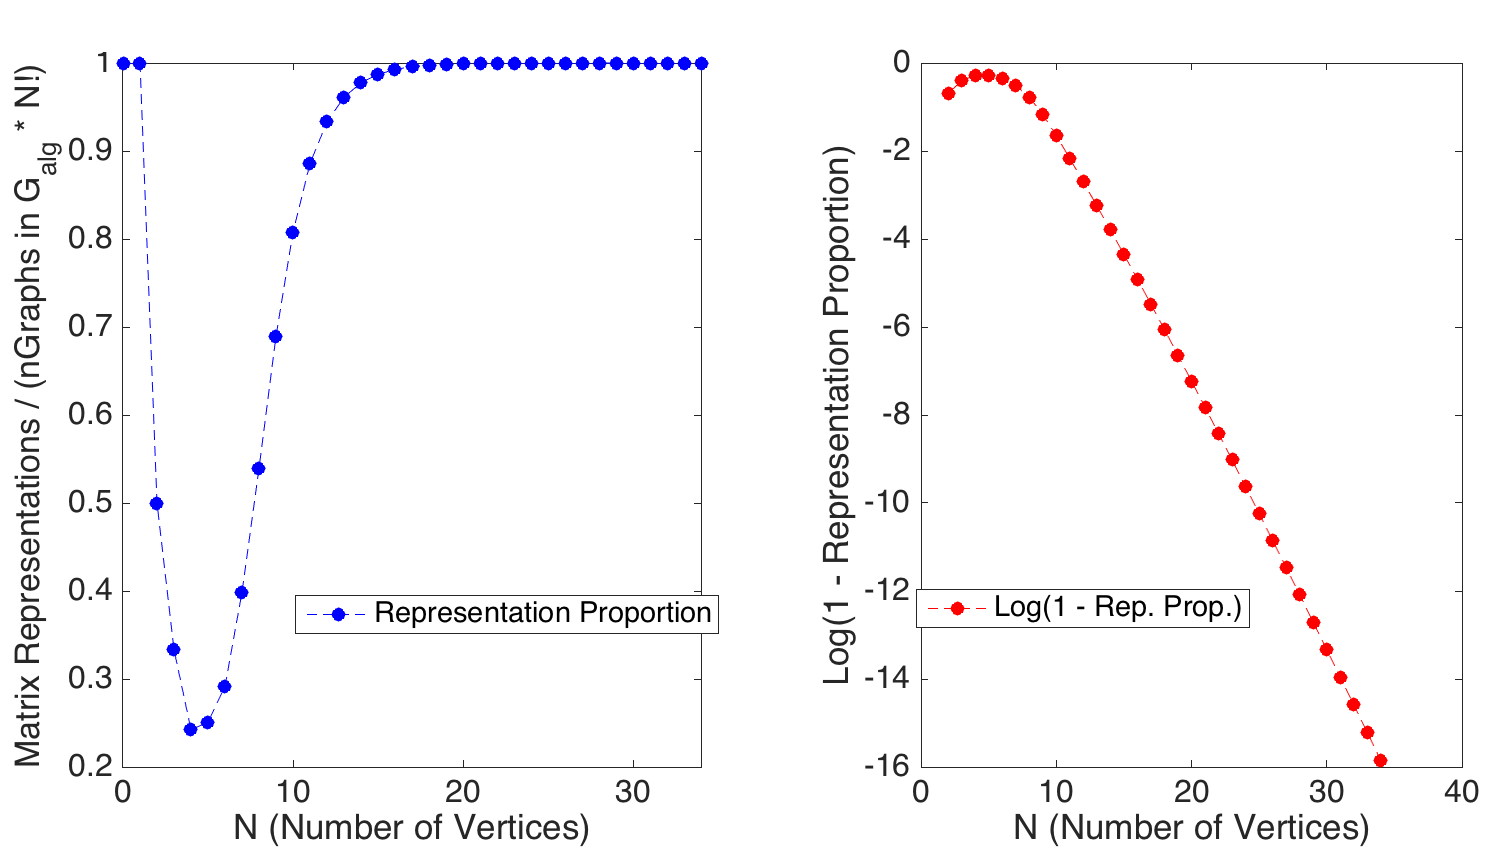
\includegraphics[width=\textwidth]{numGraphsAndMats}
\end{figure}

This should convince even a skeptical reader that for an average graph $g$ (even when treating it like an algebraic object), as $N$ increases, $\xoverline{|Aut(g)|} \rightarrow 1$.

\subsection{Implications for Perfectly Similar Vertex Sets}

Applying this back to our original purpose, we can reason that if a graph only has a single automorphism, then the only automorphism is the trivial automorphism.
Thus, the SVSes are a set of N distinct, one element sets, where each vertex is distinguishable from each other, and none share any automorphisms.
This makes checking for isomorphism between two random graphs trivial (if we have the SVSes), as the overwhelming majority of the time, we will only need to try the isomorphism implied by the direct, one to one mapping between the SVSes of the two graphs.

However, checking for Automorphisms between every single pair of vertices is clearly in a higher computational complexity class than testing for isomorphism.
Thus, we will use smart heuristics to develop quazi-similar vertex sets, which will enable us to get the benefits of SVSes (i.e. implying the isomorphisms to try) without actually proving that the automorphisms that define the SVSes exist.

\section{Quazi-Similar Vertex Sets}

Quazi-similar vertex sets are constructed with respect to a vertex invariant.
The vertex invariant is calculated for all vertices within the graph, and those with the same value are placed into the same set.
Transitivity and reflexivity clearly both hold under this definition.
Moreover, the ordering/comparability of vertex invariants gives us a natural way to order the sets within the QSVS.

In this section, we will describe how using the cycles invariant to generate QSVSes is highly successful at mirroring the true SVSes, and suggest an augmentation to cycles which correctly differentiates the two for all observed cases.



\section{Why $P^*<N$: Limitations on Cycles Usefulness}

\subsection{What is $P^*$, why does it matter?}

An ENORMOUS part of this thesis has thus far gone as assumed: what is $P$ (the maximum length cycle we are considering)?
When we are discussing cycles through a node, how long are the cycles we are considering?
The vertex invariant for cycles is clearly a vector, with the length of cycles corresponding to the place within the vector (cycles of length 2, 3, 4, etc.), but where do we draw the line?
To answer this question, I used a notion of `usefulness', to maximize the amount of information that we get out of the cycles invariant for the computation that we put into it.

Specifically, within the context of cycles as a vertex invariant, I started out with the assumption that all vertices share a single Similar Vertex Set (i.e. all are similar unless we have proof that they are not).
We then distinguish vertices by advancing P by one, we are in effect splitting this one class (or smaller classes) into smaller classes, based on the information gleaned by increasing the length of all invariant vectors by one.
This kinds of `breaking-down' leads us to a concrete notion of usefulness: for a given graph G, cycles is useful at a power $P_G$, where $P_G$ is the minimum value for P at which all of the vertex sets in the SVSes are as broken down as they can get (for any amount of P).
Thus, if we take the maximum of $P_G$ across all G, we will find a value $P^*$ at which point computation beyond this point is redundant.
This would enable us to more concretely talk about running time, and its tradeoffs.
What we find (through both computational exploration and theoretical justification) is that $P^*$ is contingent upon $N$, and specifically that:

\[ P^* = \begin{cases} 
      N-1 & \text{If N is odd} \\
      N-2 & \text{If N is even} \\
   \end{cases}
\]

\subsection{Observational Data: Diameter vs. $P_G$}

I first tried to explain $P_G$ as a function of the individual graph $G$.
Though this did not lead me anywhere directly, it did give me a clear idea of the upper bounds on $P_G$ for an individual graph.
Shown in figure \ref{fig:diamvsmaxpower} is a description of this relationship.  By no means is it rigid, but the coorelation is very strong.
It is also interesting (personally) just to see the diameter of a set of graphs laid out like this, just a side note.

\begin{figure}[h]
\label{fig:diamvsmaxpower}
\caption{\emph{Diameter Against $P_G$ with $N=9$} - The size and number next to each circle tell us how many graphs (as objects) fit into different sizes of diameter and $P_G$}
\centering
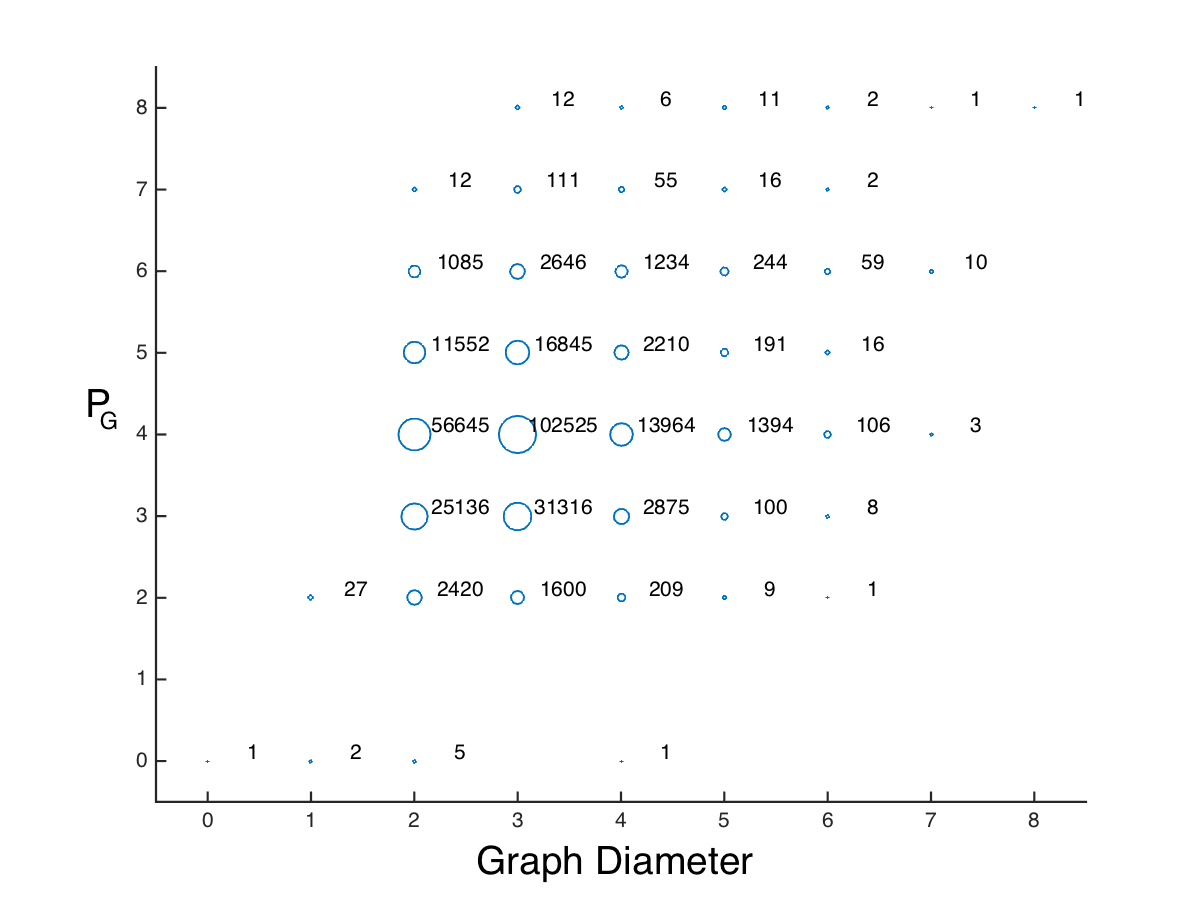
\includegraphics[width=\textwidth]{N9DiamVsDiffPower}
\end{figure}

Four things are consistent across all of the alike graphs (shown in an appendix):
\begin{itemize}
\item{There is consistently a maximum diameter for $P_G$, implying a $P^*$ for each as shown in the table below}
\item{There are never any graphs with $P_G = 1$, as we do not allow self loops }
\item{The Path graph ($P_N$), is always the lone member of the far upper right hand corner}
\item{The Cycle graph ($C_N$), always has $P_G$ equal to that of the Path graph}
\end{itemize}
The upper bound proposed by each one of the values for $P*(N)$ follows the pattern:
\[ P^* = \begin{cases} 
      N-1 & \text{If N is odd} \\
      N-2 & \text{If N is even} \\
   \end{cases}
\]
for $N <=9$. This sets up a strong case for this as a target hypothesis, but we still must prove it.

\subsection{Theoretical Justification: $P_N$ versus $C_N$}
TODO


\section{Improving upon QSVS with Flagged Cycles}

The quality of the QSVS is generally described as how close they are to the true SVSes.
In other words, quality is a measure of how frequently does a QSVS contain two or more subsets that should be independent SVSes.
Though Cycles as a vertex invariant produces QSVSes which mirror SVSes with high probability, we should examine the failures cases to see if we can do better.

We will accomplish this via a methodology I am calling `flagging' after I have seen that a few times in the literature.
Flagging (or Marking) is the process of taking a graph and appending a single vertex to it which is connected by a single edge to some target vertex in the graph.
Flagging frequently modifies graph structure enough to see impacts with solid results.

For example, if we have two co-spectral graphs, and we are curious whether or not an isomorphism exists between the two of them, we can append a flag on each one of the vertices which must be mapped together in a potential isomorphism, and then take the chromatic polynomial again.
If the new (flagged) graphs differ in their chromatic polynomial, then the two vertices that were flagged cannot have an isomorphism to one another, as modifying two isomorphic graphs in a deterministic way should preserve isomorphism.
We use this principle in the pursuit of fully differentiating a set of QSVS into a refined state that more clearly mirrors SVSes.

\subsection{Appending a Flag, Somewhat Predictable}

Our methodology for modifying the QSVSes is simple: first, calculate the QSVSes using the Cycles invariant.
For each of the sets within the QSVSes with more than one element, perform a flagging operation K times, if the set has K elements, which results in K different graphs.
Calculate the cycles graph invariant over each of these graphs.
If the cycles invariants for any two of the K graphs differs, then split apart the set of vertices into two (or more) new QSVSes, one for each different value of the graph invariant associated with the graph formed by flagging each vertex.
What a mouth-full!

An interesting piece of this is that we can actually predict some of the values that the newly created, flagged graphs, will have for their cycles invariant values.
Specifically, we can predict the number of cycles for the flag vertex, as each one of the cycles that it is a part of must go to and from the flagged vertex, and we already knew how many of those there were from the original cycles function.
Additionally, we can predict the change in the number of cycles for the flagged vertex, as we knew its cycle profile before, and the addition of a single vertex on to it can be interpreted as a recursive definition, where cycles are broken into components that travel back (and forth) from the flag vertex and those that exist within the graph.
Though difficult to explain via formulae and words, I would encourage a skeptical reader to check out my code at (/Thesis/Matlab/constituentpaths/predictPathsOfAddingOneVertex.m).

Equally interesting (to the fact that we \emph{can} predict paths for these two nodes when just given the cycles invariant) is that we \emph{cannot} make any further predictions about the flagged cycles values based solely on the plain cycles values.
We know this to be true because in co-cycles graphs, we frequently get different flagged cycles graph invariants when we flag vertices which are suggested to be isomorphic (but are not).
This is a good piece of information to know because it gives us proof that flagging is not some kind of manipulation of information that we already have, it represents a way to get pieces of information that are tangibly new.

\subsection{Intuitive Justification for Flagging}

This section is not grounded in proof, but gives a conceptual reason that flagging works at further discriminating between vertices that we think might be automorphic.
Cycles is really a rough description of the `neighborhood' of a vertex within its context in the graph.
Cycles tells us about the way that energy reverberates around a structure.
One conceptual tool I like is to think about electricity flowing (bidirectionally) around a circuit, and measuring the self-connectivity or resistance.

Flagging a node changes that dynamic.
It changes it in a way that we understand and can predict for the flagged vertex and the flag vertex.
However, it also changes the way that cycles `reverberate' through the flagged vertex, and in doing so, changes the cycles invariant at other vertices.
We can even think of this in more concrete terms: take the cycles invariant for the flagged graph (without sorting), then subtract off the cycles invariant for the non-flagged graph (again, without sorting).

This tells you exactly how many new cycles have been created which pass through the flagged node at least once.
We call this modified matrix the \emph{excess cycles} matrix.
Note that this is \emph{not} the same as the row for the flagged cycles matrix, and actually encodes significantly more information (the constituents of those paths, not only that they exist).
In doing so, we actually get tangible information about the connectivity of each of the nodes.
From the excess cycles matrix, we can calculate the distance between the flagged vertex and each of the other vertices in the graph.
We can calculate the relative makeup of each of the added cycles (how many pass through each vertex, and how many times does each double back on itself), among a large number of other features.

The intuitive justification for flagging is compelling, and if I had another month to puzzle away at this problem, this is probably the area I would spend the most time focusing on.

\subsection{Analytical Support for Flagging, and an Open Question}

The analytical support for flagging is strong:
for all graphs of size $N<=10$, cycles with flagging as a mechanism for QSVS generation correctly generated QSVSes which turned out to be the same as the SVSes.
No counterexamples were found where cycles with flagging fails to be anything short of a perfect vertex invariant.

This begs an open question: is it possible that cycles with flagging is complete as a vertex invariant?
Is it possible that this metric fully determines the automorphism sets of vertices? Maybe.
However, it is more likely (based on the raw number of graphs out there) that we have only kicked the proverbial can further down the road.
For one, the raw amount of information required in Cycles with flagging is N times the amount of information required for cycles comparison.
This alone should tell us to expect a higher threshold for failure.

That being said, there are properties that are reconstructable from excess cycles computations that make me think that flagging might have some higher order justification.
I would love to spend another few months thinking of equations that I can use to reconstruct $A$ (or better yet, determine $A$) from flagged cycles.

%\section{Limitations to Augmentation}
%\subsection{A Second Augmentation Hypothesis}